\section{Structural identification and its limits}\label{sec:identification}

\subsection{The problem}

Let $x_{it}$ collect GDP growth, the unemployment change and related variables, with
reduced-form dynamics
\[
  x_{it}=c_i+\sum_{l=1}^{p}A_l x_{i,t-l}+u_{it},\qquad \E[u_{it}u_{it}']=\Sigma .
\]
A structural model posits $u_{it}=B\varepsilon_{it}$ with mutually uncorrelated shocks
$\varepsilon_{it}$, so $\Sigma=BB'$. For any orthonormal $Q$, $BQ$ fits the data equally
well, which leaves $n(n-1)/2$ free parameters that identifying information must supply.

\paragraph{Innovations are not shocks.} Reduced-form innovations, and impulse responses
orthogonalised by an arbitrary ordering, are not structural shocks. By
equation~\eqref{eq:weighted}, a causal Okun coefficient must refer to a specific identified
shock $k$: the ratio $\kappa_k$ of its effects on unemployment and on output.

\paragraph{Strategies evaluated.} Four strategies were considered before any estimate:
\begin{itemize}
  \item \emph{Recursive orderings:} rejected. GDP and unemployment respond within the
    quarter to every shock, so no zero restriction between them is credible.
  \item \emph{Long-run restrictions} \citep{blanchard1989quah}: rejected. They assume two
    shocks and long-run neutrality, are unreliable in short samples
    \citep{faust1997longrun}, and conflate productivity with labour supply.
  \item \emph{External instruments} \citep{stock2018external}: estimated.
  \item \emph{Sign restrictions} \citep{rubio2010svar}: estimated, with inference that
    does not depend on the prior over rotations.
\end{itemize}
Local projections \citep{jorda2005lp} are an estimator, not an identification strategy.
They estimate the same responses as VARs in population \citep{plagborg2021lpvar}.

\subsection{External instruments}

\paragraph{The shocks.} Two common shocks are identified outside this study, each by
high-frequency event windows:
\begin{itemize}
  \item ECB monetary policy surprises, purged of central-bank information effects by sign
    restrictions on interest rates and stock prices
    \citep{jarocinski2020information,altavilla2019mpd};
  \item OPEC oil supply news \citep{kanzig2021oil}.
\end{itemize}
Neither is a productivity shock. No credible instrument exists for productivity or
labour-supply shocks in EU countries.

\paragraph{The local projections.} For horizon $h$, lag-augmented local projections are
estimated, pooled over countries with country effects and clustered by quarter
\citep{montielolea2021lp}:
\[
  y_{i,t+h}-y_{i,t-1}=a_i^h+b^h s_t+\sum_{l=1}^{L}\big(c_l^h s_{t-l}+d_l^{h\prime} x_{i,t-l}\big)
  +e_{it}^h .
\]
The shock-conditional ratio $\kappa(h)$ of cumulative unemployment to cumulative output
responses is estimated by LP-IV. Its Anderson--Rubin set
\citep{anderson1949ar} remains valid however weak the instrument:
\[
  \Big\{\kappa:\ (\hat b_u-\kappa\hat b_y)^2\le c^2\,\widehat{\operatorname{Var}}
  (\hat b_u-\kappa\hat b_y)\Big\}.
\]
The set is bounded exactly when the first-stage $|t|$ exceeds the critical value $c$, so an
unbounded set means the data do not determine the ratio.

\paragraph{Timing.} The shocks are monthly and are summed within each quarter, so a shock
late in a quarter has little time to act before the quarter ends. Even so, a 10 basis
point monetary tightening comes with an unemployment rate \val{id_mp_u0} percentage points
higher in the same quarter (90\% interval \val{id_mp_u0_ci}). A response that fast is
implausible for a policy shock. It points to timing within the quarter, to aggregation, or
to news about the economy contained in the policy surprise, and it is a further reason to
read these local projections cautiously.

\paragraph{Quarterly results.}
\begin{itemize}
  \item The first stages are weak: $|t|$ is at most \val{id_max_t}, against the
    conventional threshold of $3.16$ ($F=10$).
  \item All \val{id_sets} primary Anderson--Rubin sets are unbounded
    (table~\ref{tab:identification}).
  \item The quarterly sum of the oil surprise is predictable from lagged EU data
    ($p=$ \val{id_pred_oil}), which casts doubt on its exogeneity at that frequency. The
    monetary shock is not predictable ($p=$ \val{id_pred_mp}).
\end{itemize}

\paragraph{Monthly results.} A registered amendment kept the shocks at their native monthly
frequency, with monthly unemployment and industrial production as outcomes. The ratio is
then per unit of industrial production, not GDP. The primary sample was restricted to the
\val{mo_n_direct} countries whose monthly unemployment is a direct survey estimate. That restriction
defines a new assumption, that a month's value contains no later months, which a pre-shock
placebo tests.
\begin{itemize}
  \item At native frequency the oil surprise is not predictable ($p=$
    \val{mo_pred_oil}).
  \item The first stages remain weak (largest $|t|$ \val{mo_max_t}).
  \item All \val{mo_unbounded} primary sets are unbounded.
\end{itemize}

\subsection{Country-specific GDP shocks}

Identifying the effect of a country's own GDP shock requires an instrument that moves that
country's GDP and affects its unemployment only through GDP. The most defensible public
candidate is a shift-share of foreign demand
\citep{goldsmith2020bartik,borusyak2022shiftshare,adao2019shiftshare}:
\[
  Z_{it}=\sum_p e_{ip}\,g_{pt},
\]
where $e_{ip}$ is the share of country $i$'s value added absorbed in partner $p$'s final
demand \citep{oecd2025tiva} and $g_{pt}$ is partner GDP growth.

\paragraph{Partner sets.} Distant, non-European partners are the only set whose exclusion
restriction is defensible. Near partners bring migration and commuting, and intra-EU
partners share the European cycle.

\paragraph{Feasibility rule.} A registered rule required the expected first-stage $t$,
after country and quarter effects, to reach $3.16$ before any estimate. It is
\val{ss_P1_t} for distant demand. Adding near partners raises it only to \val{ss_P2_t}, and
intra-EU partners to \val{ss_P3_t}, while making exclusion indefensible. The design was
therefore not estimated.

\subsection{Sign restrictions}

\paragraph{The model.} A pooled panel VAR in GDP growth, deflator inflation and the changes
in unemployment and participation set-identifies three shocks by impact signs, following
the logic of \citet{foroni2018laborsupply}:
\begin{itemize}
  \item demand: $g+$, $\pi+$, $\Delta u-$;
  \item technology: $g+$, $\pi-$, $\Delta u-$;
  \item labour supply: $\pi-$, $\Delta u+$, $\Delta p+$.
\end{itemize}
The restriction on unemployment under technology is debatable: in sticky-price models,
employment can fall after a productivity improvement \citep{gali1999technology}. A
registered robustness check drops it.

\paragraph{Inference.} The usual uniform prior over rotations shapes the reported responses
\citep{baumeister2015sign}. We therefore report the identified set for every posterior draw
of the reduced form, summarised by the robust Bayesian approach of
\citet{giacomini2021robust}.

\paragraph{Results.}
\begin{itemize}
  \item \emph{Plausibility.} Every posterior draw admits the impact restrictions
    (\val{sr_nonempty}). Imposed also one quarter later, they are admissible in only
    \val{sr_nonempty_h01} of draws, so the data contradict that variant.
  \item \emph{Demand against technology.} The demand and technology sets for the Okun
    ratio are \val{sr_sets}. Demand- and technology-driven ratios cannot be distinguished.
  \item \emph{Why the ratios are unbounded.} This outcome is close to guaranteed by the
    design. The signs restrict impact responses only, and the ratio divides by the
    cumulative GDP response, whose admissible set includes zero (at eight quarters, for
    demand, \val{sr_dem_gdp8_ci}). The result shows that these restrictions are
    uninformative about the ratio; it is not evidence about the ratio's size. Bounds on
    elasticities or narrative sign restrictions would be the next step.
  \item \emph{Labour supply against demand.} They differ at impact only because the
    signs impose it. By eight quarters both robust regions for the unemployment response
    include zero. The robust region for each shock's share of the forecast-error variance
    of the quarterly change in unemployment (the VAR variable, not the level) runs from
    \val{sr_dem_fevd_lo} to \val{sr_dem_fevd_hi} for demand and from \val{sr_ls_fevd_lo}
    to \val{sr_ls_fevd_hi} for labour supply.
  \item \emph{The uniform prior.} It gives sharp-looking ratios (demand \val{sr_dem_uniform},
    technology \val{sr_tech_uniform}), but the sharpness comes from the prior, not from the
    data (figure~\ref{fig:sign}).
  \item \emph{Recursive orderings.} Reported only as a measure of sensitivity, the
    \val{sr_n_orderings} orderings move the orthogonalised ``GDP shock'' ratio between \val{sr_order_min_h4}
    and \val{sr_order_max_h4} at four quarters, depending on whether GDP is ordered before
    unemployment. None of them is causal.
\end{itemize}

\subsection{Testable and untestable assumptions}

\paragraph{Testable.}
\begin{itemize}
  \item instrument relevance (first-stage strength);
  \item predictability of a shock from lagged data, a partial test of exogeneity;
  \item the timing of monthly series (placebo);
  \item the joint compatibility of sign restrictions with the reduced form (non-emptiness).
\end{itemize}

\paragraph{Not testable.}
\begin{itemize}
  \item event-window exogeneity;
  \item the purity of the monetary shock;
  \item the exclusion restriction of foreign demand;
  \item the sign restrictions themselves;
  \item linearity and homogeneity of responses.
\end{itemize}

\subsection{A post-hoc check of the pandemic window}

The registered rules drop an observation if any period of its variables lies in
2020--2021. The quarterly window starts at $t-4$, the monthly window at $t-12$ and the VAR
window at $t-2$. The change at the longest lag, however, is measured from the level one
period earlier, which can fall in 2021 while the observation is kept. After an external
review we widened every window by one period. This check was not registered, and the
registered results remain primary:
\begin{itemize}
  \item quarterly: the largest first-stage $|t|$ is \val{ws_q0_max_t} with the registered
    window and \val{ws_q1_max_t} with the widened one, and \val{ws_q1_unbounded} sets
    remain unbounded;
  \item monthly: \val{ws_m0_max_t} and \val{ws_m1_max_t}, with \val{ws_m1_unbounded} sets
    unbounded;
  \item sign restrictions: every draw remains admissible (\val{ws_sr_nonempty}), and the
    demand and technology Okun-ratio regions are \val{ws_sr_regions}.
\end{itemize}
No conclusion changes.

\subsection{What the identification study shows}

With the public data available for the \eu, the instruments and restrictions we could
defend are uninformative about a causal Okun coefficient. That is a statement about these
designs, not about the size of any causal effect. Every coefficient in this study
therefore remains a reduced-form association. More informative answers would need:
\begin{itemize}
  \item utilisation-adjusted quarterly productivity series;
  \item quasi-experimental variation in labour supply;
  \item country-specific policy shocks, such as narrative fiscal shocks;
  \item regional data;
  \item longer break-free samples.
\end{itemize}

% Generated by eu-okun publication. Do not edit.
\begin{table}[t]\centering\small
\caption{First-stage strength and Anderson--Rubin (Fieller) 90\% sets of the shock-conditional ratio of unemployment to output responses. Quarterly: output is GDP; monthly: industrial production. Shift-share: benchmark expected first-stage $t$ (no estimate). The conventional weak-instrument threshold is $|t|=3.16$. Two rays: the union of two unbounded half-lines.}
\label{tab:identification}
\begin{tabular}{lllrl}
\toprule
Design & Instrument & Horizon & First-stage $t$ & 90\% AR set \\
\midrule
Quarterly LP-IV & ECB monetary policy & 4 quarters & $-0.64$ & unbounded \\
Quarterly LP-IV & ECB monetary policy & 8 quarters & $+0.02$ & two rays \\
Quarterly LP-IV & OPEC oil supply news & 4 quarters & $+1.27$ & unbounded \\
Quarterly LP-IV & OPEC oil supply news & 8 quarters & $+0.70$ & unbounded \\
Monthly LP-IV & ECB monetary policy & 12 months & $-0.22$ & unbounded \\
Monthly LP-IV & ECB monetary policy & 24 months & $+0.34$ & unbounded \\
Monthly LP-IV & OPEC oil supply news & 12 months & $+1.21$ & unbounded \\
Monthly LP-IV & OPEC oil supply news & 24 months & $+0.75$ & unbounded \\
Shift-share & distant demand & --- & $0.19$ & not estimated \\
Shift-share & + near extra-EU & --- & $0.31$ & not estimated \\
Shift-share & intra-EU leave-one-out & --- & $0.66$ & not estimated \\
\bottomrule
\end{tabular}
\end{table}


\begin{figure}[t]\centering
\begin{minipage}{0.49\textwidth}\centering
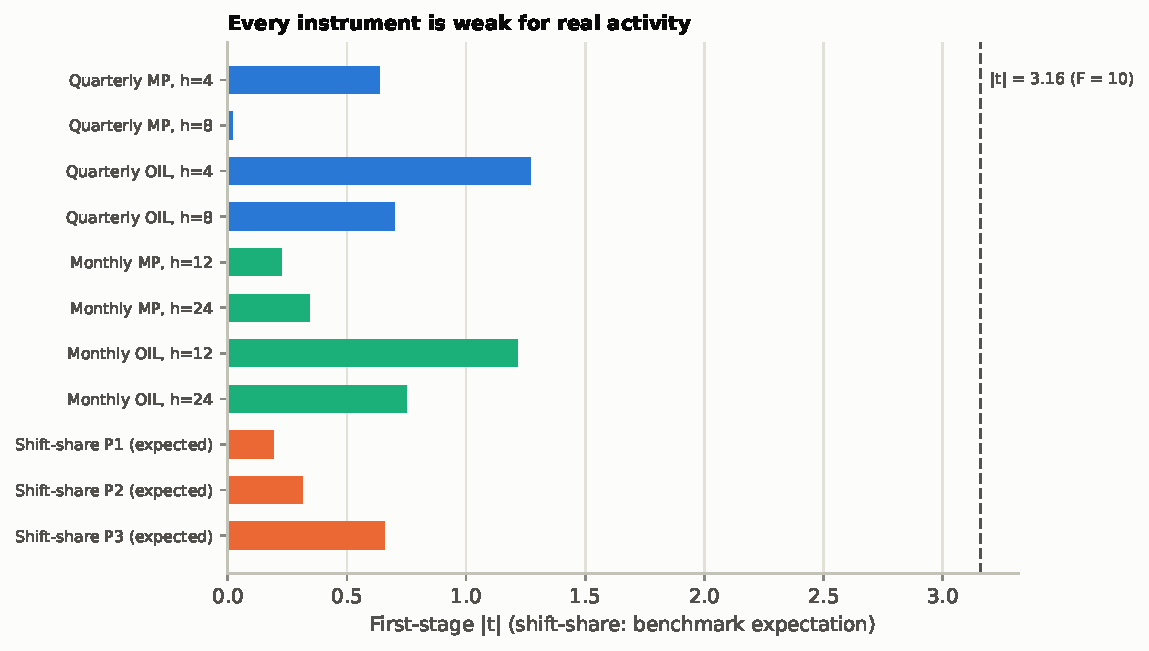
\includegraphics[width=\textwidth]{fig4_identification.pdf}
\end{minipage}\hfill
\begin{minipage}{0.49\textwidth}\centering
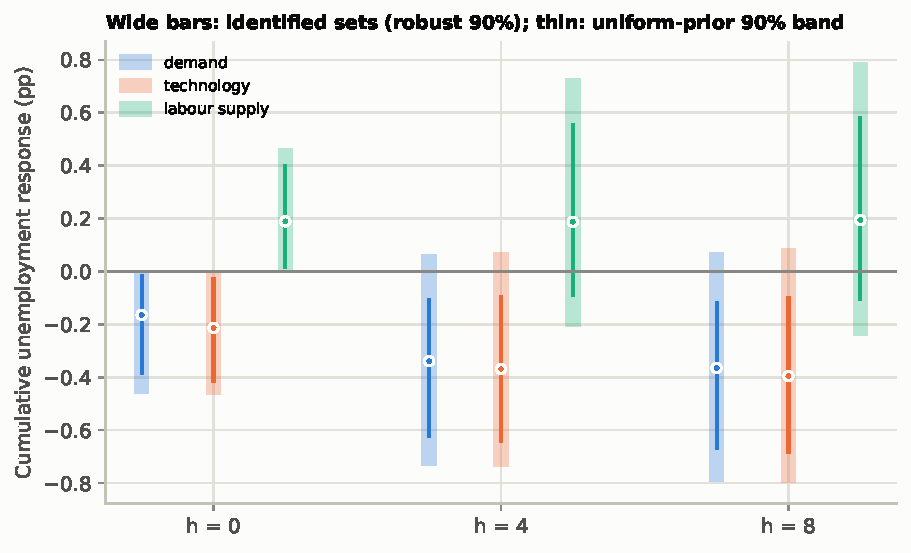
\includegraphics[width=\textwidth]{fig5_sign_restrictions.pdf}
\end{minipage}
\caption{Left: first-stage strength of every instrument (shift-share: benchmark
expectation); the dashed line is $|t|=3.16$. Right: cumulative unemployment responses to
one-standard-deviation shocks. Wide bars are robust 90\% regions of the identified sets;
thin lines and dots are the uniform-rotation posterior 90\% bands and medians.}
\label{fig:sign}
\end{figure}
